\section{内核功能实现}\label{sec:KernelFunctionalityImplementation}

内核是操作系统的核心组件,负责管理内存和设备,同时为软件应用程序提供使用这些资源的接口。根据复杂性和目标的不同,内核的开发可以遵循不同的模型。主要有两种模型:微内核\footnote{微内核是一种操作系统内核设计,其核心理念是将内核功能最小化,只保留最基本的操作系统服务,如最低级的内存管理、进程调度和通信机制。其他更复杂的服务,如文件系统、网络协议、设备驱动等,则运行在用户空间。}和宏内核\footnote{宏内核则是传统的内核设计方式,将大部分的系统服务和管理功能,如设备驱动、文件系统管理、网络服务等,都直接在内核空间内实现。}。微内核的目标是将大多数服务运行在用户空间,从而提高安全性和模块化。

MinmusOS 采用的是宏内核模式,因此其所有服务和设备驱动程序都在单一地址空间内运行,并处于特权模式下。这种模式提高了效率并减少了代码复杂性,但缺点是其中任何一个组件的错误都可能导致整个系统崩溃。

在本节(\cref{sec:KernelFunctionalityImplementation})中,笔者将详细探讨 MinmusOS 内核各项功能的实现,包括中断管理、驱动程序、多任务处理、系统调用、命令行解释器、内存管理以及文件系统。

\subsection{中断(Interrupts)}

中断是操作系统中关键的概念之一,主要用于处理外部设备的信号或内部事件。中断机制使得CPU可以响应并处理紧急事件,同时保持对其他任务的执行。中断主要分为三种类型:

\begin{enumerate}
    \item \textbf{异常(Exceptions)}:同步中断,由CPU执行指令过程中的事件或错误引发,例如除以零错误、执行非法指令或访问无效内存地址。异常通常分为两类:可屏蔽异常和不可屏蔽异常。可屏蔽异常允许操作系统根据当前的需求和优先级来决定是否立即处理。
    \item \textbf{硬件中断(Hardware Interrupts)}:异步中断,由外部硬件设备产生,例如键盘输入、鼠标移动或网络数据包到达。硬件中断使得设备可以通知CPU它们需要立即处理的事件,这对于实时数据处理非常重要。
    \item \textbf{软件中断(Software Interrupts)}:由执行特定的CPU指令集(如INT指令)显式触发,常用于操作系统的系统调用,比如文件访问、网络通信或其他服务请求。软件中断还可以用来执行BIOS(基本输入输出系统)例程,或者其他低级操作。
\end{enumerate}

当中断发生时,CPU会采取以下步骤来处理:

\begin{enumerate}
    \item \textbf{保存当前状态}:CPU首先保存当前正在执行的任务的状态,以便中断处理完成后可以恢复。
    \item \textbf{识别中断类型}:CPU通过查询中断向量表(一个存储了所有中断处理程序入口地址的表格)来识别中断的具体类型和来源。
    \item \textbf{执行中断服务例程(ISR,Interrupt Service Routine)}:每种中断类型都有对应的服务程序。CPU执行这些程序来处理中断。
    \item \textbf{恢复状态}:中断服务完成后,CPU恢复之前中断的任务状态,继续之前的操作。
\end{enumerate}

中断处理机制的设计对于操作系统的效率和响应时间至关重要。优秀的中断处理策略可以显著提高系统的整体性能和用户体验。

\subsubsection{中断描述符表(Interrupt Descriptor Table)}

中断描述符表(IDT)是x86架构中特有的一个关键数据结构,用于管理中断的处理。它的主要目的是提供一个中断服务例程(ISR)的地址映射,当中断发生时,CPU能够知道跳转到哪个位置执行相应的中断处理程序。

IdtEntry 是中断描述符表(IDT)中的基本单元,它定义了每个中断处理函数的具体属性和位置。IdtEntry 结构体的定义如\cref{lst:IdtEntryDataStructure}所示。\texttt{\#[derive(Copy, Clone, Debug)]} 使用 derive 宏为结构体自动实现 Copy、Clone 和 Debug 这三个 trait,\texttt{\#[repr(C, packed)]} 用于指定结构体使用 C 语言风格的内存布局并取消字段对齐,以确保字段在内存中紧凑排列。

\begin{listing}[htbp]
    \begin{minted}{rust}
#[derive(Copy, Clone, Debug)]
#[repr(C, packed)]
pub struct IdtEntry {
    offset_low: u16,       // 偏移地址的低 16 位
    segment_selector: u16, // 中断处理程序代码所在的段选择器
    reserved: u8,          // 保留字段,设置为 0
    flags: u8,             // 位标志
    offset_high: u16,      // 偏移地址的高 16 位
}
    \end{minted}
    \caption{\texttt{IdtEntry}数据结构}\label{lst:IdtEntryDataStructure}
\end{listing}

位标志,包含门类型(Gate Type)、DPL(Descriptor Privilege Level)和 P(Presence):

\begin{enumerate}
    \item \textbf{门类型(Gate Type)}:决定IDT条目是中断门还是陷阱门。例如,0xE(1110b)代表32位中断门。
    \item \textbf{DPL(Descriptor Privilege Level)}:指定可以调用中断的最低特权级(CPL),通常为0,表示只有内核模式可以使用。
    \item \textbf{P(Presence)}:此位必须设置为1,表示此中断向量是有效的。
\end{enumerate}

IdtEntry 结构体提供了 set 方法(\cref{lst:IdtEntrySetMethod})用于设置中断处理程序的地址,这个方法接受一个32位的整数 offset,代表中断处理程序的地址。然后将这个地址分解为两个16位的部分,分别存储到 offset\_low 和 offset\_high。

\begin{listing}[htbp]
    \begin{minted}{rust}
pub fn set(&mut self, offset: u32) {
    self.offset_low = ((offset << 16) >> 16) as u16;
    self.offset_high = (offset >> 16) as u16;
}
    \end{minted}
    \caption{\texttt{IdtEntry}的set方法}\label{lst:IdtEntrySetMethod}
\end{listing}

IdtDescriptor 结构体(\cref{lst:IdtDescriptorDataStructure})定义了一个用于加载中断描述符表(IDT)的描述符。它用于指定 IDT 的大小和内存中的位置,从而允许处理器正确地找到并使用 IDT。size 表示 IDT 的大小,但实际上是 IDT 中最后一个有效条目的偏移量加一。因为中断向量表的条目索引从 0 开始,所以 size 字段的值等于 IDT 的字节长度减一。offset 是一个指向 InterruptDescriptorTable 的指针,表示 IDT 的起始物理地址。这个指针告诉处理器从哪里开始读取中断向量表的数据。

\begin{listing}[htbp]
    \begin{minted}{rust}
#[repr(C, packed)]
pub struct IdtDescriptor {
    size: u16,
    offset: *const InterruptDescriptorTable,
}
    \end{minted}
    \caption{\texttt{IdtDescriptor}数据结构}\label{lst:IdtDescriptorDataStructure}
\end{listing}

InterruptDescriptorTable 结构体(\cref{lst:InterruptDescriptorTableDataStructure})实现了一个关键的系统级数据结构,即中断描述符表(IDT)。这个表是操作系统中管理中断向量的核心结构,用于定义每个中断或异常的处理程序地址。

\begin{listing}[htbp]
    \begin{minted}{rust}
#[repr(C, packed)]
pub struct InterruptDescriptorTable {
    entries: [IdtEntry; IDT_ENTRIES],
}

impl InterruptDescriptorTable {
    pub fn init(&mut self) {
        for i in 0..IDT_ENTRIES {
            self.add(i, exceptions::generic_handler as u32);
        }
    }

    pub fn add(&mut self, int: usize, handler: u32) {
        self.entries[int].set(handler);
    }

    pub fn load(&self) {
        let descriptor = IdtDescriptor {
            size: (IDT_ENTRIES * size_of::<IdtEntry>() - 1) as u16,
            offset: self,
        };
        unsafe {
            asm!("lidt [{0:e}]", in(reg) &descriptor);
        }
    }

    pub fn add_exceptions(&mut self) {
        self.add(0x00, exceptions::division_error as u32);
        ...
        self.add(0x15, exceptions::control_protection_exception as u32);
    }
}
    \end{minted}
    \caption{\texttt{InterruptDescriptorTable}数据结构}\label{lst:InterruptDescriptorTableDataStructure}
\end{listing}

中断描述符表(IDT)的结构体定义与方法实现:

\begin{enumerate}
    \item \textbf{结构体定义}:entries 包含了 IDT\_ENTRIES(256)数量的 IdtEntry 结构体实例。每个 IdtEntry 对应一个中断向量,存储中断处理程序的具体位置和相关属性。
    \item \textbf{init方法}:初始化 IDT 的每个条目,将所有中断向量的处理程序设置为一个通用的处理函数 \texttt{exceptions::generic\_handler}。
    \item \textbf{add方法}:设置特定中断向量的处理程序。它接受中断向量的索引和处理程序的地址(函数指针),然后调用 IdtEntry 的 set 方法来更新相应的条目。
    \item \textbf{load方法}:将 IDT 加载到 CPU 的 IDT 寄存器。它创建一个 IdtDescriptor 结构体,该结构体包含了 IDT 的大小和地址,然后使用 lidt 汇编指令加载这个描述符。
    \item \textbf{add\_exceptions方法}:为常见的 CPU 异常配置特定的处理程序,如除零错误、无效操作码、双重故障、通用保护和页面错误等,中断向量表见\cref{tab:InterruptVectorTable}。
\end{enumerate}

IDT\_ENTRY 是 IdtEntry 类型的静态变量,\cref{lst:IdtEntryTemplate}定义了一个默认的 IDT 条目模板。这个模板被用来初始化 IDT 数组中的每个条目。

\begin{listing}[htbp]
    \begin{minted}{rust}
pub static IDT_ENTRY: IdtEntry = {
    // 段选择器,确定中断处理程序的代码段
    let segment_selector: u16 = {
        let rpl = 0b00 << 0;       // 请求特权级(Ring Privilege Level),0 表示最高权限级别
        let ti = 0b0 << 2;         // 表指示符(Table Indicator),0 表示使用全局描述符表(GDT)
        let index = 0b1 << 3;      // GDT 中的索引,这里是 0x8
        rpl | ti | index           // 组合成完整的段选择器
    };

    // 保留字段,必须设为 0
    let reserved: u8 = 0;

    // 标志位字段,定义了 IDT 条目的属性
    let flags: u8 = {
        let gate_type = 0xe << 0;  // 门类型,0xE 表示 32 位中断门,0xF 表示 32 位陷阱门
        let zero = 0 << 3;         // 保留位,必须为 0
        let dpl = 0 << 5;          // 描述符特权级,0 表示只有内核模式可以使用此中断
        let p = 1 << 7;            // 存在位(Presence bit),1 表示此中断有效
        gate_type | zero | dpl | p // 组合成完整的标志位
    };

    // 构造 IdtEntry 结构体实例
    IdtEntry {
        offset_low: 0,             // 中断处理程序的低 16 位地址,初始化设置为 0,后续指定具体值
        segment_selector,          // 上面定义的段选择器
        reserved,                  // 保留位,始终为 0
        flags,                     // 标志位,定义了 IDT 条目的特性
        offset_high: 0,            // 中断处理程序的高 16 位地址,初始化设置为 0,后续指定具体值
    }
};
    \end{minted}
    \caption{IDT 条目模板}\label{lst:IdtEntryTemplate}
\end{listing}

IDT 是 InterruptDescriptorTable 类型的静态变量,它实际上是一个包含 256 个 IdtEntry 条目的数组。这个数组构成了整个中断描述符表,用于响应各种中断请求。\cref{lst:IDT}使用 IDT\_ENTRY 来初始化每个元素,这意味着每个条目初始时都复制了 IDT\_ENTRY 的设置。特定的中断向量将通过调用 InterruptDescriptorTable 的 add 方法来设置特定的处理函数。

\begin{listing}[htbp]
    \begin{minted}{rust}
pub static mut IDT: InterruptDescriptorTable = InterruptDescriptorTable {
    entries: [IDT_ENTRY; IDT_ENTRIES]
};
    \end{minted}
    \caption{中断描述符表}\label{lst:IDT}
\end{listing}

IDT 定义了操作系统如何响应硬件和软件生成的中断。每个条目对应一个中断向量,系统在收到中断时会查询 IDT 以确定如何处理该中断。通过提供一个统一的方式来处理所有类型的中断,操作系统能够更加有效地管理资源和响应外部事件,从而增强系统的稳定性和响应性。

\subsubsection{中断服务例程(Interrupt Service Routines)}

中断服务例程(ISR)是一种特定的程序,用于处理来自硬件或软件的中断信号。当系统发生中断时,CPU 会自动查找中断描述符表(IDT)中相应的服务例程,并跳转到该例程执行相关操作。与普通的 C 函数不同,ISR 由 CPU 直接调用,并使用特定的 iret 指令返回,这种指令用于恢复中断前的状态,确保系统能安全地继续执行其他任务。

在编写 ISR 时,需要特别注意 CPU 在调用中断服务例程之前会自动将一些寄存器的值压栈,这些寄存器包括 EFLAGS、EIP 和 CS。EFLAGS 寄存器包含了系统的状态标志,EIP 是程序计数器,指示下一条执行指令的地址,CS 是代码段寄存器,指示当前执行代码的段基址。

大部分操作系统使用专门的汇编语言函数来实现中断处理程序,以确保处理过程的高效和准确。MinmusOS 采用 Rust 的内联汇编技术来实现 ISR。这种方法允许在中断服务例程中直接调用其他 Rust 函数,然后通过 iret 指令安全返回,这种技术的使用使得中断处理程序既可以保持高效,也能利用 Rust 语言的安全特性。

\begin{listing}[htbp]
    \begin{minted}{rust}
#[naked]
pub extern "C" fn generic_handler() {
    unsafe {
        asm!(
        "push 0xFF",              // 向堆栈推送一个错误代码
        "call exception_handler", // 调用 exception_handler 函数,用于显示错误信息并处理中断
        "add esp, 4",             // 调整堆栈指针,以清除之前压入的错误代码
        "iretd",                  // 使用中断返回指令,恢复之前由 CPU 自动保存的状态
        options(noreturn),        // 表明汇编代码块执行后不会返回到原始的 Rust 函数中
        );
    }
}
    \end{minted}
    \caption{通用中断处理器}\label{lst:GenericHandler}
\end{listing}

\cref{lst:GenericHandler}定义了一个用于处理多种中断的通用中断服务例程(ISR)。使用 \texttt{\#[naked]} 属性表示这个函数没有由编译器生成的 prologue \footnote{函数的 prologue 是函数实际执行之前的准备阶段。在这个阶段,编译器或者程序会保存旧的基指针、设置新的基指针和为局部变量分配空间。}和 epilogue\footnote{函数的 epilogue 是函数执行完成后的清理阶段。在这个阶段,编译器或者程序会恢复堆栈指针、恢复基指针和返回到调用者。},使得函数可以完全控制所有的堆栈操作。这种处理方式对于中断处理程序来说是必要的,因为它们需要精确控制寄存器和堆栈的状态,但也增加了复杂性和出错的风险。

\begin{listing}[htbp]
    \begin{minted}{rust}
#[no_mangle]
pub extern "C" fn exception_handler(int: u32, eip: u32, cs: u32, eflags: u32) {
    unsafe {
        PRINTER.set_colors(COLOR_WHITE, COLOR_BLUE);
        PRINTER.clear();
    }
    lib::println!();
    lib::println!("  ========== MinmusOS v1.0 ==========                            By Jishen Lin");
    lib::println!();
    lib::println!("  SERIOUS KERNEL ERROR!");
    lib::println!();
    lib::println!("  MinmusOS has encountered a fatal error and the system has been halted.");
    lib::println!();
    lib::println!();
    lib::println!();
    lib::println!();
    lib::println!("  EXCEPTION DESCRIPTION:");
    lib::println!();
    match int {
        0x00 => {
            lib::println!("    DIVISION ERROR!");
        }
        ...
        _ => {
            lib::println!("    EXCEPTION!");
        }
    }
    lib::println!();
    lib::println!();
    lib::println!("  TECHNICAL INFORMATION:");
    lib::println!();
    lib::println!("    ERROR_CODE      : {}", int);
    lib::println!("    INSTRUCTION_PTR : 0x{:X}", eip);
    lib::println!("    CODE_SEGMENT    : 0x{:X}", cs);
    lib::println!("    EXTENDED_FLAGS  : 0b{:b}", eflags);
    lib::println!();
    lib::println!();
    lib::print!("  Please restart your computer. :)");
    loop {}
}
    \end{minted}
    \caption{异常处理器}\label{lst:ExceptionHandler}
\end{listing}

在调试过程中,在代码中通过内联汇编使用 int 命令可以手动触发中断。\cref{lst:ExceptionHandler}为 MinmusOS 提供了友好的用户交互(\cref{fig:ExceptionHandlerPresentation})。蓝屏界面采用了经典的蓝底白字风格,类似于传统的Windows蓝屏死机(BSOD),并显示了详细的错误信息,包括错误类型和技术信息(如错误代码、指令指针、代码段、扩展标志等),有助于开发人员定位问题,便于调试和修复。

\begin{figure}[htbp]
    \centering
    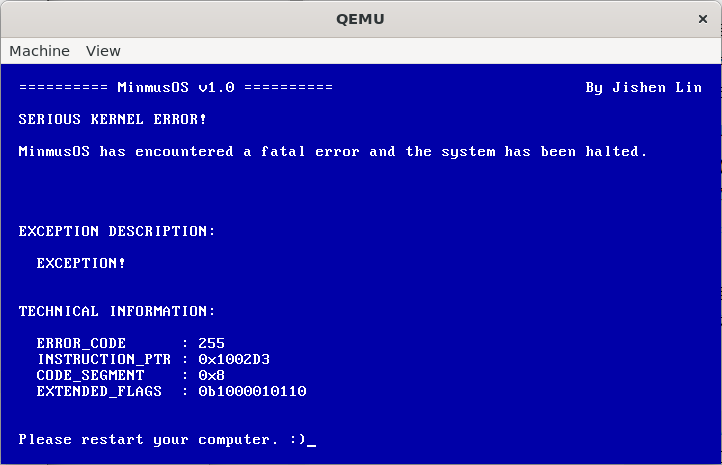
\includegraphics[width=0.8\textwidth]{figures/ExceptionHandlerPresentation.png}
    \caption{异常处理器演示}
    \label{fig:ExceptionHandlerPresentation}
\end{figure}

\subsubsection{CPU 异常(CPU Exceptions)}

异常是 CPU 在执行当前指令过程中遇到错误时自身触发的一种中断。在 x86 架构上,大约有 20 种不同的 CPU 异常类型,见\cref{tab:InterruptVectorTable}。\cref{tab:InterruptVectorTable} 参考自 Intel® 64 和 IA-32 架构软件开发者手册。

\begin{longtable}[c]{@{}llllll@{}}
    \caption{中断向量表}
    \label{tab:InterruptVectorTable}                                                                                                                                                                                                                  \\
    \toprule
    \textbf{向量} & \textbf{助记符} & \textbf{描述}                                                                                                                                            & \textbf{类型} & \textbf{错误代码} & \textbf{来源}                   \\ \midrule
    \endfirsthead
    \multicolumn{6}{r}{\textbf{续表~\thetable}}                                                                                                                                                                                                         \\
    \toprule
    \textbf{向量} & \textbf{助记符} & \textbf{描述}                                                                                                                                            & \textbf{类型} & \textbf{错误代码} & \textbf{来源}                   \\ \midrule
    \endhead
    \hline
    \multicolumn{6}{r}{续下页}
    \endfoot
    \endlastfoot
    0           & \#DE         & 除零错误                                                                                                                                                   & 故障          & 否             & DIV 和 IDIV 指令                 \\
    1           & \#DB         & 调试异常                                                                                                                                                   & 故障/陷阱       & 否             & 指令、数据和 I/O 断点;单步执行等           \\
    2           &              & NMI中断                                                                                                                                                  & 中断          & 否             & 不可屏蔽的外部中断                     \\
    3           & \#BP         & 断点                                                                                                                                                     & 陷阱          & 否             & INT3 指令                       \\
    4           & \#OF         & 溢出                                                                                                                                                     & 陷阱          & 否             & INTO 指令                       \\
    5           & \#BR         & BOUND 范围超出                                                                                                                                             & 故障          & 否             & BOUND 指令                      \\
    6           & \#UD         & 无效操作码(未定义操作码)                                                                                                                                          & 故障          & 否             & UD 指令或保留操作码                   \\
    7           & \#NM         & 设备不可用(无数学协处理器)                                                                                                                                         & 故障          & 否             & 浮点数或 WAIT/FWAIT 指令            \\
    8           & \#DF         & 双重故障                                                                                                                                                   & 中止          & 是(零)          & 任何能生成异常、NMI 或 INTR 的指令        \\
    9           &              & 协处理器段溢出(保留)                                                                                                                                            & 故障          & 否             & 浮点数指令                         \\
    10          & \#TS         & 无效的 TSS\footnote{TSS(Task State Segment)是Intel x86架构中用于任务切换和状态维护的数据结构。它存储了处理器在执行任务时需要的所有状态信息,使得操作系统能够管理多任务环境中的任务切换。TSS的使用主要体现在硬件级别的任务切换和保护模式下的任务状态管理。} & 故障          & 是             & 任务切换或 TSS 访问                  \\
    11          & \#NP         & 段不存在                                                                                                                                                   & 故障          & 是             & 加载段寄存器或访问系统段                  \\
    12          & \#SS         & 栈段故障                                                                                                                                                   & 故障          & 是             & 栈操作和 SS 寄存器加载                 \\
    13          & \#GP         & 通用保护                                                                                                                                                   & 故障          & 是             & 任何内存引用和其他保护检查                 \\
    14          & \#PF         & 页面错误                                                                                                                                                   & 故障          & 是             & 任何内存引用                        \\
    15          &              & (Intel 保留)                                                                                                                                             &             & 否             &                               \\
    16          & \#MF         & x87 FPU 浮点错误(数学故障)                                                                                                                                     & 故障          & 否             & x87 FPU 浮点或 WAIT/FWAIT 指令     \\
    17          & \#AC         & 对齐检查                                                                                                                                                   & 故障          & 是(零)          & 内存中的任何数据引用                    \\
    18          & \#MC         & 机器检查                                                                                                                                                   & 中止          & 否             & 错误代码(如果有)和来源取决于模型             \\
    19          & \#XM         & SIMD 浮点异常                                                                                                                                              & 故障          & 否             & SSE/SSE2/SSE3 浮点指令            \\
    20          & \#VE         & 虚拟化异常                                                                                                                                                  & 故障          & 否             & EPT 违规                        \\
    21          & \#CP         & 控制保护异常                                                                                                                                                 & 故障          & 是             & RET/IRET/RSTORSSP/SETSSBSY 指令 \\
    22-31       &              & (Intel 保留)                                                                                                                                             &             &               &                               \\
    32-255      &              & 用户定义(非保留)中断                                                                                                                                            & 中断          &               & 外部中断或 INT n 指令                \\ \bottomrule
\end{longtable}

\subsubsection{可编程中断控制器(Programmable Interrupt Controller)}

可编程中断控制器(Programmable Interrupt Controller,简称 PIC),尤指 8259 PIC,是早期计算机主板上用于管理硬件中断的一个小型芯片。在现代计算机中,这一芯片通常已被整合进 CPU 的设计中。PIC 的核心作用是接收来自硬件设备的中断信号,并在 CPU 准备接收时,将这些信号有效地分派给 CPU,从而响应外部设备的事件或请求。

PIC 有 28 个引脚,其中 8 个引脚是中断输入线,用于连接那些可以触发中断的硬件组件。这些中断线路将外部设备如键盘、鼠标或其他I/O设备的中断请求直接传输到 PIC。由于单个 PIC 只能处理有限的 8 个中断,现代计算机系统为了扩展中断处理能力,通常会使用两个 PIC 芯片,配置为一主一从模式。这种配置允许系统处理更多的中断线路,总共可达 15 个中断(一个用于连接主从 PIC)。虽然现代计算机系统普遍采用了更为先进的高级可编程中断控制器(APIC),以支持更大数量的中断线路和更复杂的中断管理功能,PIC 依旧因其向后兼容性而被支持在新的系统中,确保老旧硬件和软件的正常运行。

CPU 在设计时已经为处理器内部的异常(如除零错误、访问违规等)预留了前 32 个中断向量。因此,来自外部硬件的中断必须被映射到 32 号以上的中断向量,以避免与这些处理器异常冲突。

重新映射中断是通过向 PIC 的命令和数据端口发送特定的命令来完成的。对于主 PIC,其命令端口位于 0x20,数据端口位于 0x21;从 PIC 的命令端口位于 0xA0,数据端口位于 0xA1。初始化 PIC 时,会发送一个初始化命令,设定中断向量的偏移量,指定哪个是主 PIC,哪个是从 PIC,并设置运行模式。

可编程中断控制器(Programmable Interrupt Controller)驱动程序的实现见\cref{sec:ProgrammableInterruptControllerDriver}。

\subsection{驱动程序(Drivers)}

设备驱动程序是一种软件组件,其目的是使特定的硬件设备与内核进行接口交互。默认情况下,操作系统并不知道如何与硬件通信,因此需要驱动程序将操作系统的请求转换成硬件能够理解和执行的命令。

\subsubsection{可编程中断控制器驱动程序(Programmable Interrupt Controller Driver)}\label{sec:ProgrammableInterruptControllerDriver}

kernel/src/drivers/pic.rs 定义了一个用于管理可编程中断控制器(Programmable Interrupt Controller,PIC)的驱动程序,特别针对老式的 8259 PIC 设计。这些 PICs 主要用于中断管理,使得硬件中断能被适当地映射并处理。

常量定义如下:

\begin{enumerate}
    \item \texttt{MASTER\_PIC\_COMMAND\_PORT}:主 PIC 接收命令的端口地址是 0x20
    \item \texttt{MASTER\_PIC\_DATA\_PORT}:主 PIC 数据读写的端口地址是 0x21
    \item \texttt{SLAVE\_PIC\_COMMAND\_PORT}:从 PIC 接收命令的端口地址是 0xA0
    \item \texttt{SLAVE\_PIC\_DATA\_PORT}:从 PIC 数据读写的端口地址是 0xA1
    \item \texttt{COMMAND\_INIT}:用于初始化 PIC 的命令字节,其值为 0x11
    \item \texttt{COMMAND\_EOF}:用于告诉 PIC 中断处理完成的命令字节,其值为 0x20
    \item \texttt{MODE}:设置 PIC 的工作模式为 8086 模式,其值为 0x01
    \item \texttt{OFFSET}:定义中断向量表中断向量的起始偏移量,这里设为 32,这是因为 0-31 号中断已被 CPU 的异常占用
    \item \texttt{IRQ\_COUNT}:每个 PIC 能够处理的中断数量,这里设为 8,表示每个 PIC 可以管理 8 个中断
\end{enumerate}

\cref{lst:MasterSlavePICInstance}定义了一个名为 PICS 的静态变量,它是 Pics 类型的实例,代表系统中的主从可编程中断控制器(PIC)。该实例包括两个 Pic 结构体,分别配置了主和从 PIC 的中断偏移量、命令端口和数据端口。此静态变量在整个程序运行期间全局可访问,用于初始化和管理硬件中断,确保操作系统能够正确响应外部设备的中断请求。

\begin{listing}[htbp]
    \begin{minted}{rust}
pub static PICS: Pics = Pics {
    master: Pic {
        offset: OFFSET,
        command_port: MASTER_PIC_COMMAND_PORT,
        data_port: MASTER_PIC_DATA_PORT,
    },
    slave: Pic {
        offset: OFFSET + IRQ_COUNT,
        command_port: SLAVE_PIC_COMMAND_PORT,
        data_port: SLAVE_PIC_DATA_PORT,
    },
};
    \end{minted}
    \caption{主从可编程中断控制器(PIC)实例}\label{lst:MasterSlavePICInstance}
\end{listing}

\cref{lst:PicDataStructure}定义了一个可编程中断控制器(PIC)的基本属性和操作方法。这个结构体和其方法主要用于对硬件中断进行低级控制,允许操作系统正确地响应外部中断请求。

\begin{listing}[htbp]
    \begin{minted}{rust}
struct Pic {
    offset: u8,       // 中断向量的起始偏移量,这个偏移量是中断向量表中该 PIC 控制的中断开始位置
    command_port: u8, // PIC 的命令端口地址
    data_port: u8,    // PIC 的数据端口地址
}

impl Pic {
    // 从 PIC 的数据端口读取一个字节的数据
    pub fn read_data(&self) -> u8 {
        let data: u8;
        unsafe {
            asm!("in al, dx", out("al") data, in("dx") self.data_port as u16);
        }
        data
    }

    // 将数据写入到 PIC 的数据端口
    pub fn write_data(&self, data: u8) {
        unsafe {
            asm!("out dx, al", in("dx") self.data_port as u16, in("al") data);
        }
    }

    // 向 PIC 的命令端口发送指定的命令
    pub fn send_command(&self, command: u8) {
        unsafe {
            asm!("out dx, al", in("dx") self.command_port as u16, in("al") command);
        }
    }

    // 通知 PIC 一个中断处理已经结束
    pub fn end_interrupt(&self) {
        unsafe {
            asm!("out dx, al", in("dx") self.command_port as u16, in("al") COMMAND_EOF);
        }
    }

    // 检查给定的中断号是否由当前的 PIC 处理,判断依据是中断号是否位于该 PIC 的控制范围内
    pub fn handles_interrupt(&self, interupt: u8) -> bool {
        self.offset <= interupt && interupt < self.offset + IRQ_COUNT
    }
}
    \end{minted}
    \caption{\texttt{Pic}数据结构}\label{lst:PicDataStructure}
\end{listing}

\cref{lst:PicsDataStructure}定义了一个包含两个可编程中断控制器(PIC),即主 PIC 和从 PIC 的组合。该结构体及其方法的设计与实现主要用于系统中断管理,允许系统初始化和管理来自硬件的中断信号。

\begin{listing}[htbp]
    \begin{minted}{rust}
pub struct Pics {
    master: Pic, // 主 PIC
    slave: Pic,  // 从 PIC
}

impl Pics {
    // 初始化
    pub fn init(&self) {
        // 读取当前的中断屏蔽状态
        let mask1 = self.master.read_data();
        let mask2 = self.slave.read_data();
        // 向每个 PIC 发送初始化命令
        self.master.send_command(COMMAND_INIT);
        wait();
        self.slave.send_command(COMMAND_INIT);
        wait();
        // 设置偏移量
        self.master.write_data(self.master.offset);
        wait();
        self.slave.write_data(self.slave.offset);
        wait();
        // 向主 PIC 发送一个数值 4,表示从 PIC 通过主 PIC 的 IRQ2 连接,配置主 PIC 知道如何与从 PIC 通信
        self.master.write_data(4);
        wait();
        // 向从 PIC 发送一个数值 2,指定它是通过主 PIC 的 IRQ2 接入的,为从 PIC 配置连接到主 PIC 的方式
        self.slave.write_data(2);
        wait();
        // 配置为 8086 模式
        self.master.write_data(MODE);
        wait();
        self.slave.write_data(MODE);
        wait();
        // 最终恢复初始屏蔽状态
        self.master.write_data(mask1);
        self.slave.write_data(mask2);
    }

    // 检查指定的中断号是否由当前 Pics 实例的主或从 PIC 处理。此方法为中断服务例程提供决策支持,决定是否需要响应某个特定中断
    pub fn handles_interrupt(&self, interrupt: u8) -> bool {
        self.master.handles_interrupt(interrupt) || self.slave.handles_interrupt(interrupt)
    }

    // 通知 PIC 中断处理已经结束。如果从 PIC 处理了中断,则先通知从 PIC,然后无论如何都通知主 PIC
    pub fn end_interrupt(&self, interrupt: u8) {
        if self.handles_interrupt(interrupt) {
            if self.slave.handles_interrupt(interrupt) {
                self.slave.end_interrupt();
            }
            self.master.end_interrupt();
        }
    }
}
    \end{minted}
    \caption{\texttt{Pics}数据结构}\label{lst:PicsDataStructure}
\end{listing}

在与硬件通信时,尤其是在初始化或配置硬件如可编程中断控制器(PIC)时,必须确保在发送连续的配置命令之间有足够的时间间隔,让硬件有机会响应每个命令。wait 函数(\cref{{lst:PicWaitFunction}})通过向一个通常未使用的端口(0x80)写入一个值(通常是0),来创造一个小的延时,这样的操作需要硬件访问时间,从而实现延迟的目的。

\begin{listing}[htbp]
    \begin{minted}{rust}
pub fn wait() {
    unsafe {
        asm!("out dx, al", in("dx") 0x80u16, in("al") 0u8);
    }
}
    \end{minted}
    \caption{wait函数}\label{lst:PicWaitFunction}
\end{listing}

设计与实现考量:

\begin{enumerate}
    \item \textbf{安全与底层访问}:由于直接与硬件端口交互,多数操作都在 unsafe 块中执行,这符合 Rust 的安全原则,仅在必要时放宽规则。
    \item \textbf{中断管理}:Pics 结构体及其方法设计考虑了中断的优先级和处理流程,确保系统对中断的响应既快速又正确。
    \item \textbf{灵活性和扩展性}:通过独立控制每个 PIC,系统可以灵活地配置中断处理,适应不同的硬件和系统需求。
\end{enumerate}

\subsubsection{键盘驱动程序(Keyboard Driver)}








\subsubsection{高级技术附件磁盘驱动程序(Advanced Technology Attachment Disk Driver)}

\subsection{多任务处理(Multitasking)}

\subsubsection{上下文切换(Context Switching)}

\subsubsection{CPU 调度器(CPU Scheduler)}

\subsubsection{任务管理器(Task Manager)}

\subsection{系统调用(System Calls)}

\subsection{命令行解释器(Shell)}

\subsection{内存管理(Memory Management)}

\subsection{文件系统(File System)}